% !TEX root = ../main.tex
\newpage
\section{\mywork Emerging Network Topologies}
\subsection{\STDP applied to networks of theta neurons}
%\textcolor{red}{TODO}: \textsl{explain in detail how the different methods \cref{eq:KempterSTDPFormulation2,eq:SongSTDPFormulation} will be implemented, using \STDP coupled with \IP.}

Following the 


\subsection{Rescaling \texorpdfstring{$W_K$}{TEXT}}
We decided to scale all learning windows presented in Chapter \ref{sec:HebbianLearningAndSynapticPlasticity} to the same order of magnitude, to make for a fair comparison of the learning dynamics over time. What is left now is to tune the hyperparameters $w^{\mathrm{in}}$ and $w^{\mathrm{out}}$.
\begin{figure}[H]
\centering
\includegraphics[height = \textheight]{../Figures/Learning/KempterWinWout.pdf}
\caption{Tuning of the hyperparameters $w^{\mathrm{in}}$ and $w^{\mathrm{out}}$. Left: the learning dynamics with zero}
\label{fig:STDP}
\end{figure}


\subsection{Results}

\begin{figure}[H]
\centering
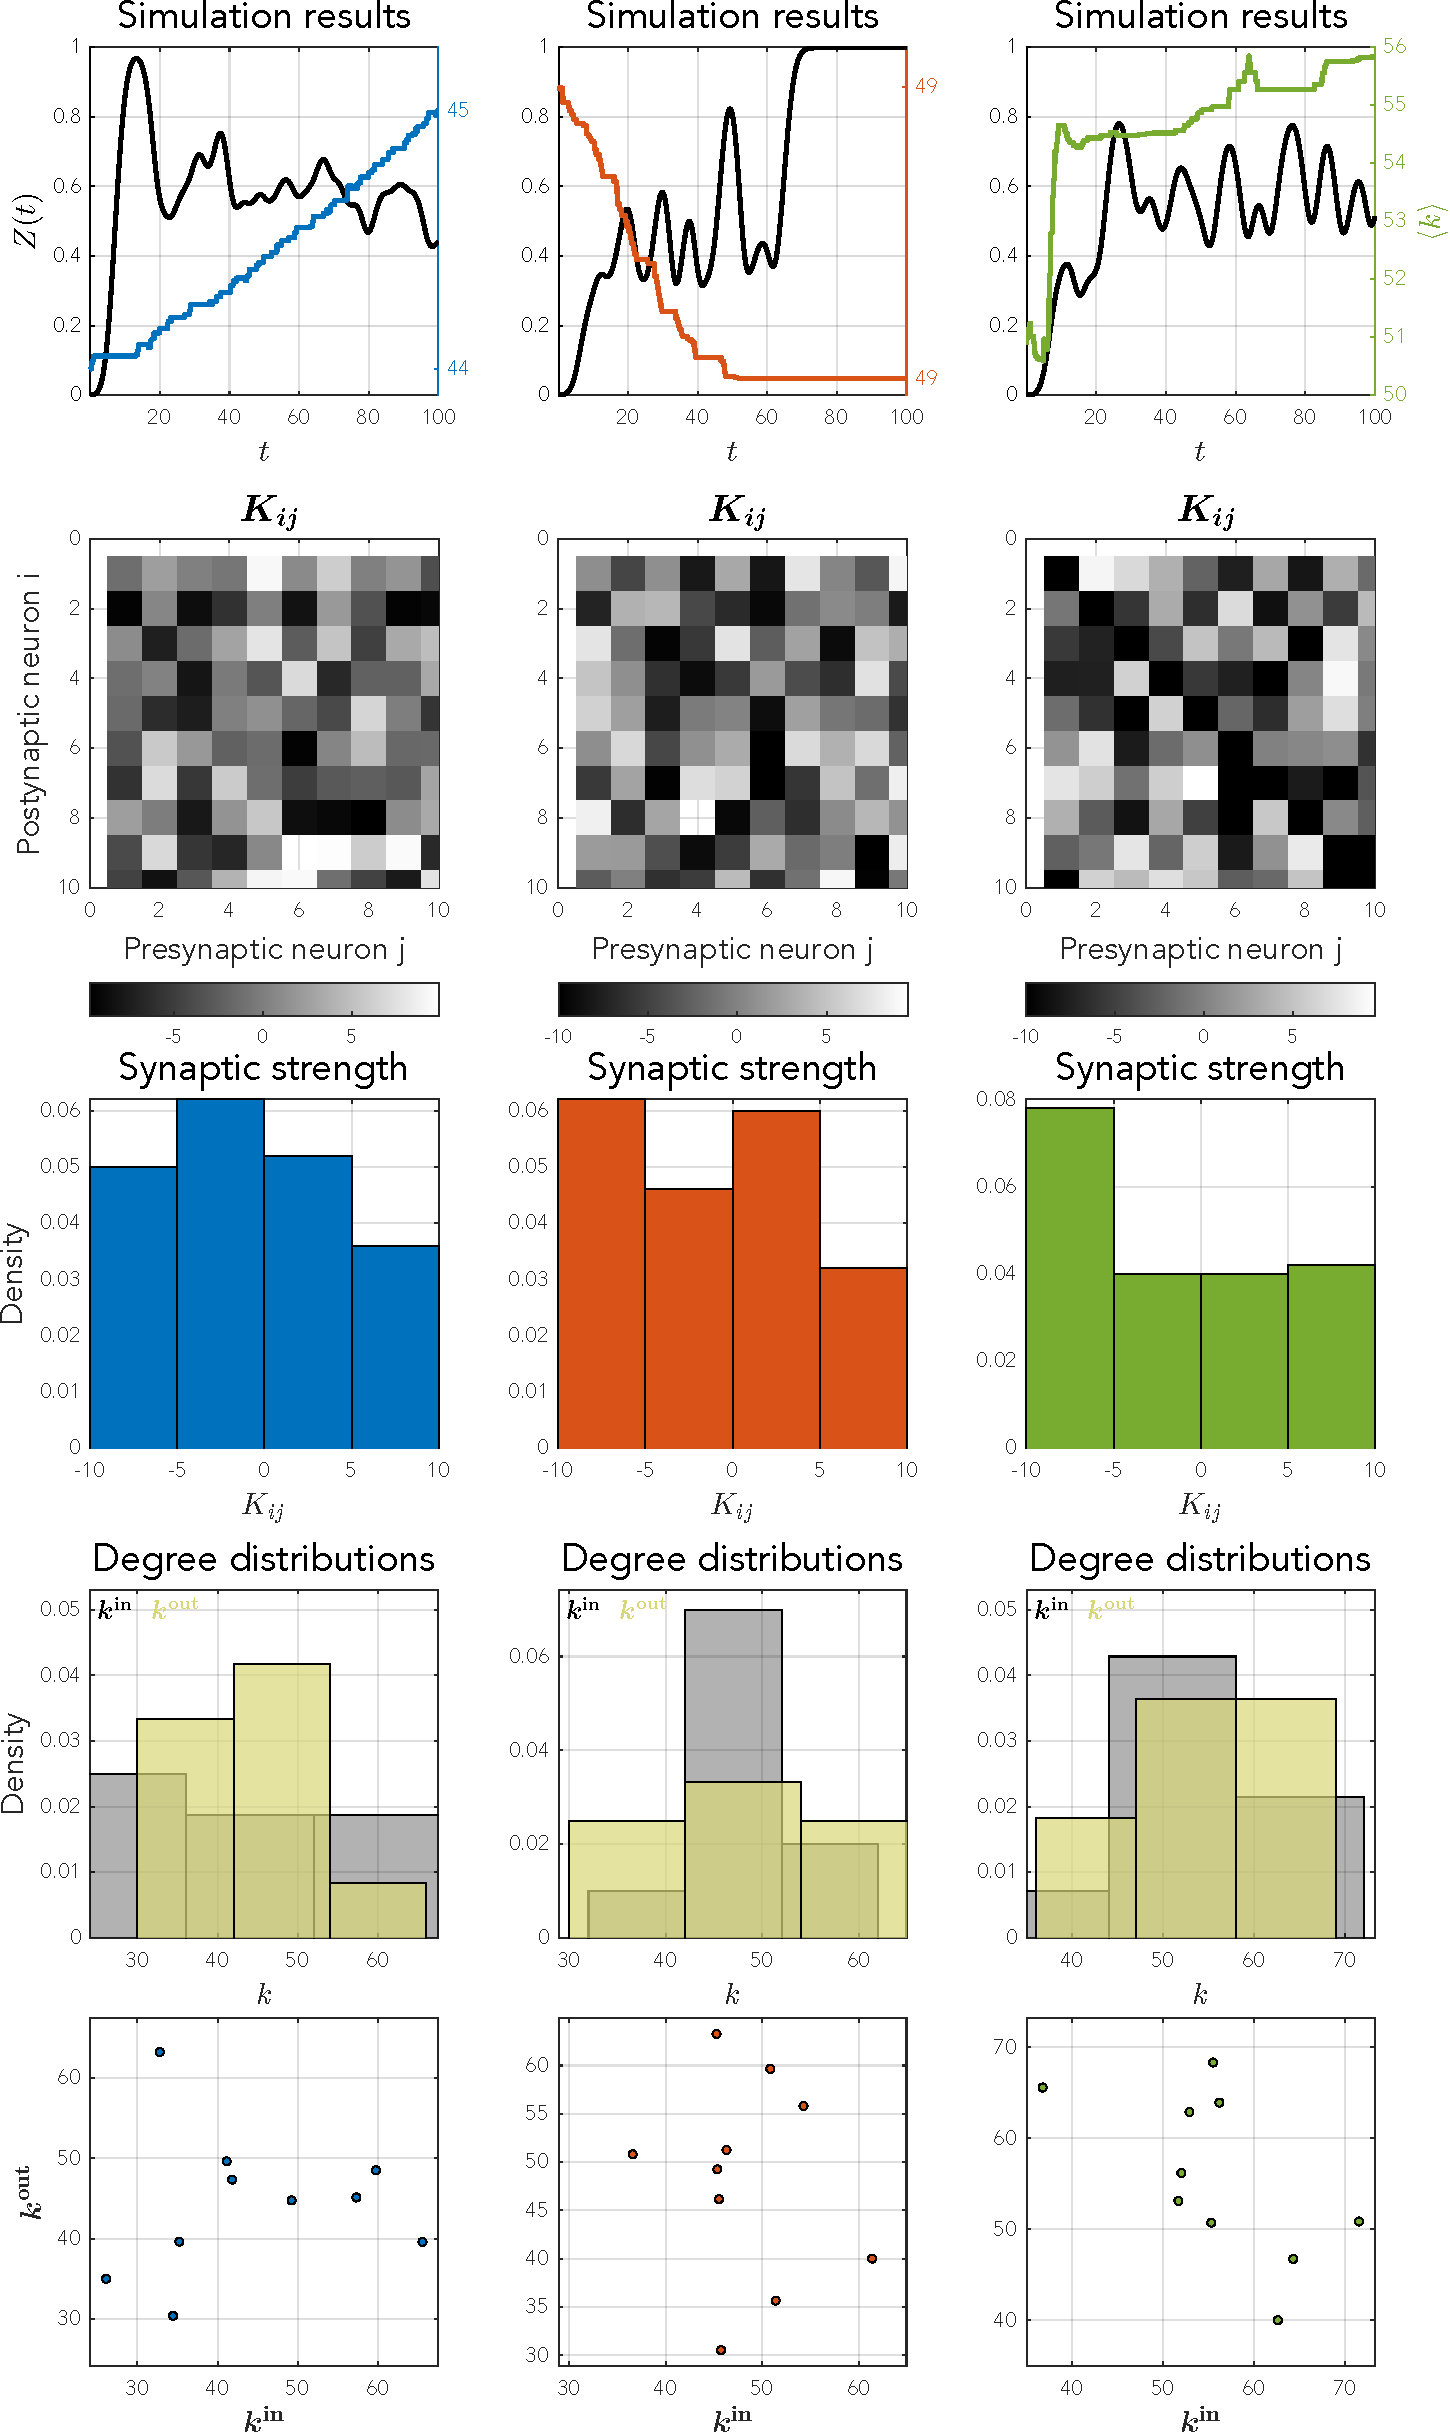
\includegraphics[height = \textheight]{../Figures/Learning/STDP.pdf}
\caption{Results of the \STDP learning.}
\label{fig:STDP}
\end{figure}

\begin{figure}[H]
\centering
\includegraphics[height = \textheight]{../Figures/Learning/STDPandIP.pdf}
\caption{Results of the \STDP learning with \IP learning.}
\label{fig:STDP}
\end{figure}

\subsection{Results}
\textcolor{red}{TODO}: \textsl{describe the emergent behaviour.}

